\section{Topic Tree}
\subsection{Overview}
Most learning management systems do not have a simple and easy method to import course material and resources from other courses. Some LMS platforms such as OpenLearning have no method of importing any data at all, and other platforms such as Canvas allows you to import crowd sourced material into your own course, however still does not allow you to import topics of resources. \\

This new LMS will have a new topic tree feature, which will allow teachers and academics to add course material under a specific topic instead.\\
Each topic will have prequisites of other topics, for example the topic Graphs will be a prequisite for the topic Depth first Search.\\

\begin{figure}[h!]
    \centering
    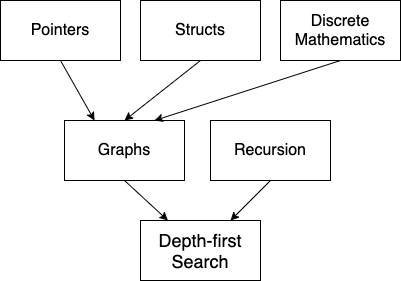
\includegraphics[scale=0.4]{topic-tree-example}
    \caption{Example of a topic tree with Depth first search}
\end{figure}

In the above example, pointers, structs and discrete mathematics must be learned in order to learn graphs. Likewise, graphs and recursion is required to learn depth first search.\\
\\
Specific courses in this new LMS would be created by choosing the topics this new course has, and all course materials under each topic would be imported into the respective topic. This allows for faster creation of courses, and course materials can be reused more easily.\\

\subsection{Requirements}
The requirements below are draft requirements, and will become more specific throughout the next stages of the thesis.\\
Each requirement will have a priority: High, Medium or Low. High priority requirements will be completed first, and then medium and low priority requirements respectively. \\

\subsection{Functional Requirements}

\textbf{Viewing Topics}
\begin{enumerate}
\item Users can view and navigate topics
    \begin{enumerate}
    \item Users can view groups of topics \textcolor{Orange}{Medium}
    \item Users can view topics within each group \textcolor{Red}{High}
    \item Users can search for a topic \textcolor{Red}{High}
    \item Users can 
    \end{enumerate}
\end{enumerate}

\textbf{Adding Topics and resources}

\textbf{Deleting Topics}

\textbf{Topic Prequisites}

\textbf{Exporting}
